\documentclass{article}
\title{Assignment 4}
\usepackage{hyperref}
\usepackage{graphicx}
\graphicspath{{./images/}}

\begin{document}
    \title{%
    Assignment 4 \\
    \large CSE235
    }
    
    \author{Daniël de Weerd - 4962699 \\
    Wouter Büthker - 5061717
    }
    
    \maketitle
    
    \section{}
    \subsection{}
    \begin{verbatim}
        wbuthker@W-PC:~$ telnet www.weer.nl 80
        Trying 52.49.153.133...
        Connected to b2cwebsite-live-lb-960116390.eu-west-1.elb.amazonaws.com.
        Escape character is '^]'.
        HEAD /regenradar/nederland HTTP/1.1
        host: www.weer.nl

        HTTP/1.1 200 OK
        Age: 459
        Cache-Control: max-age=600
        Content-Type: text/html; charset=utf-8
        Date: Sat, 21 Dec 2019 15:46:35 GMT
        Server: nginx/1.16.0
        Vary: Accept-Encoding
        Via: 1.1 varnish-v4
        X-Cache: HIT
        X-Powered-By: PHP/5.5.26
        X-Varnish: 507558504 507075416
        Connection: keep-alive

     \end{verbatim}

     \subsection{}
     It does not load the map and it shows the html header at the top of the page

     \subsection{}
     The website is served from a web cache between the host and the user

     \subsection{}
     The maximum age of the cache before it has to do a new request to the host

     \section{}
     \subsection{}

     If the field is too small it only sends the characters within the specified length.
     If the field is too large it will return a 400 bad request and it will keep waiting until the character limit is reached.

     \section{}
     \subsection{}

     No because of local caching

     \subsection{}

     Because the username and password have to be send with every request the page now denies access (401).

     \section{}
     \subsection{}
     Connect 4

     \subsection{}
     \url{https://basisonderwijs.online/digibordtools/vieropeenrij.html}

     A positive aspect of this game is that it is very clear who's turn it is, there is no noise or clutter. A negative aspect is that the game doesn't look very good.

     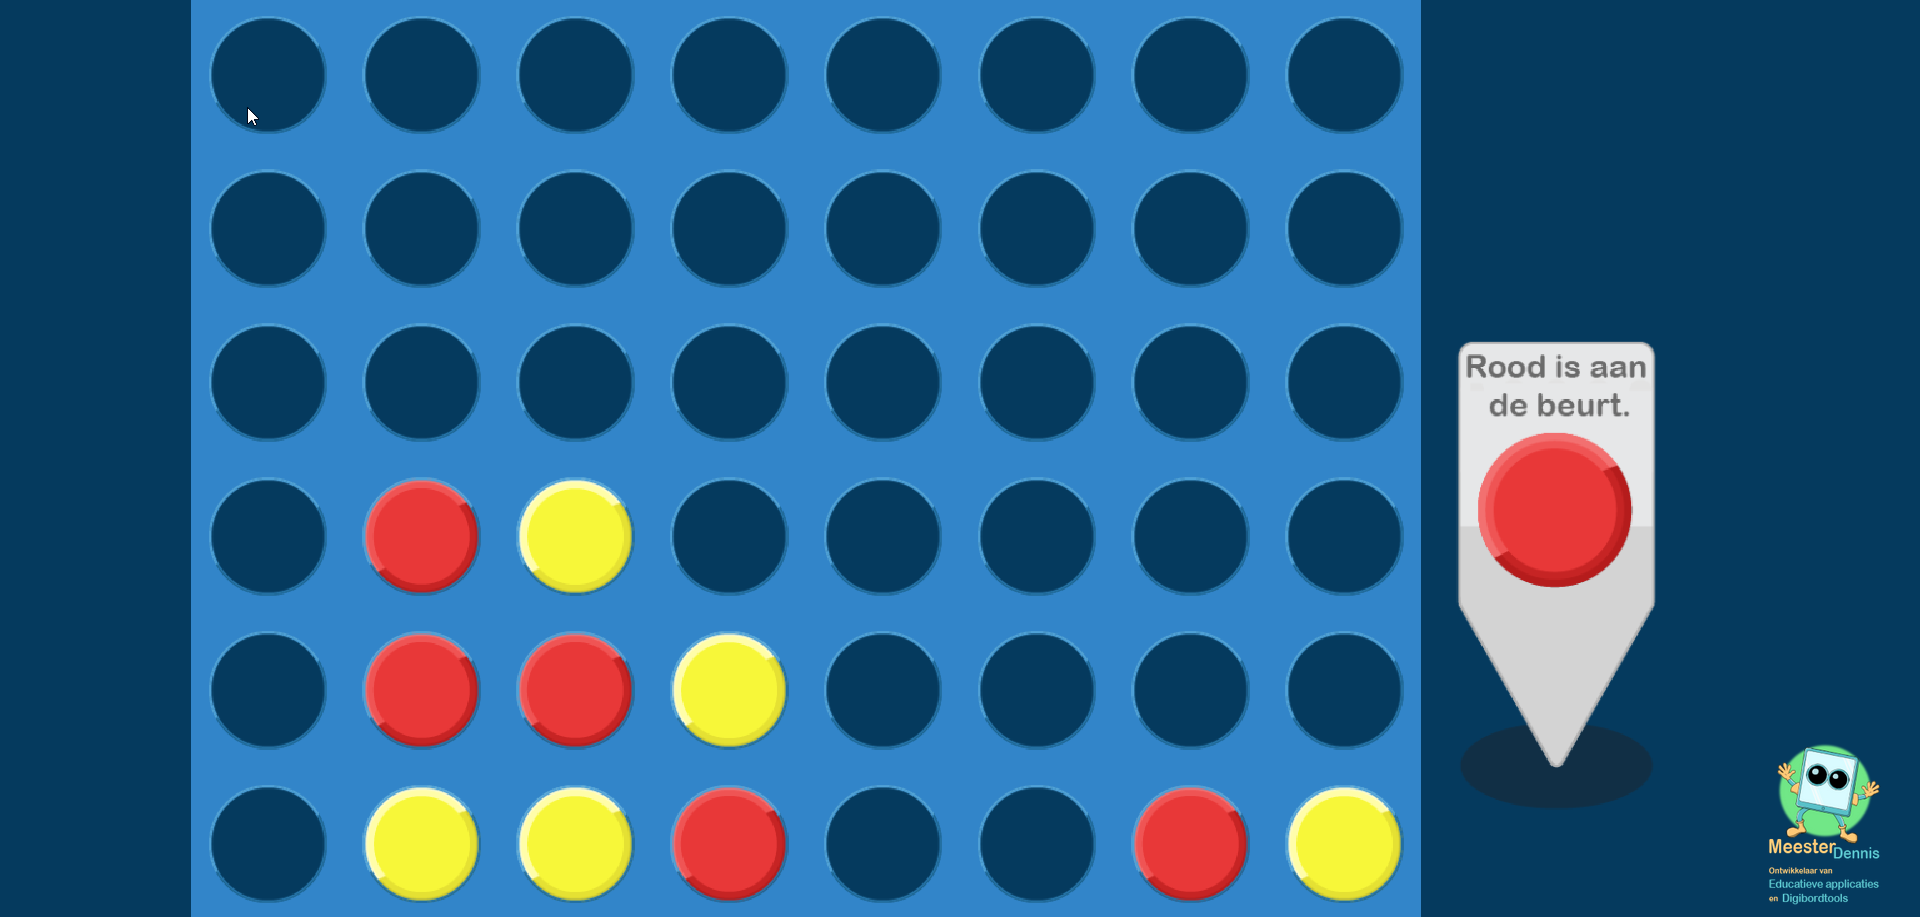
\includegraphics[width=\linewidth]{3}



     \url{https://www.spelletjes.nl/spel/4-op-een-rij}

    A positive aspect of this game is that it looks good. A negative aspect is that it is not very clear who's turn it is and what is supposed to happen.

     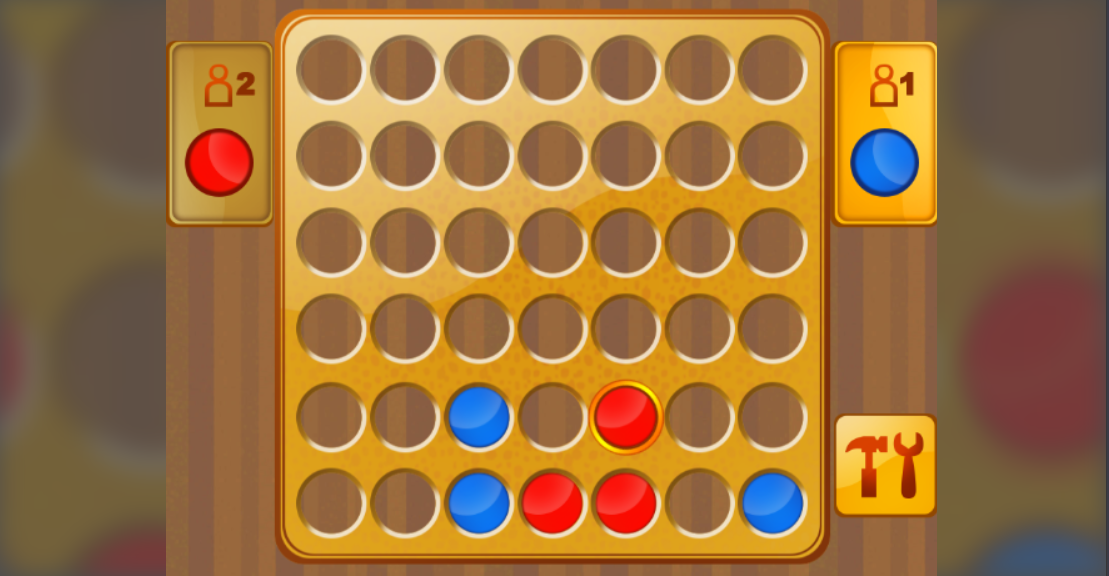
\includegraphics[width=\linewidth]{1}


     A positive aspect of this game is that it is clear who's turn it is and how long it has taken. A negative aspect is that looks kind of bland.

     \url{https://www.funnygames.nl/spel/connect_4.html}

     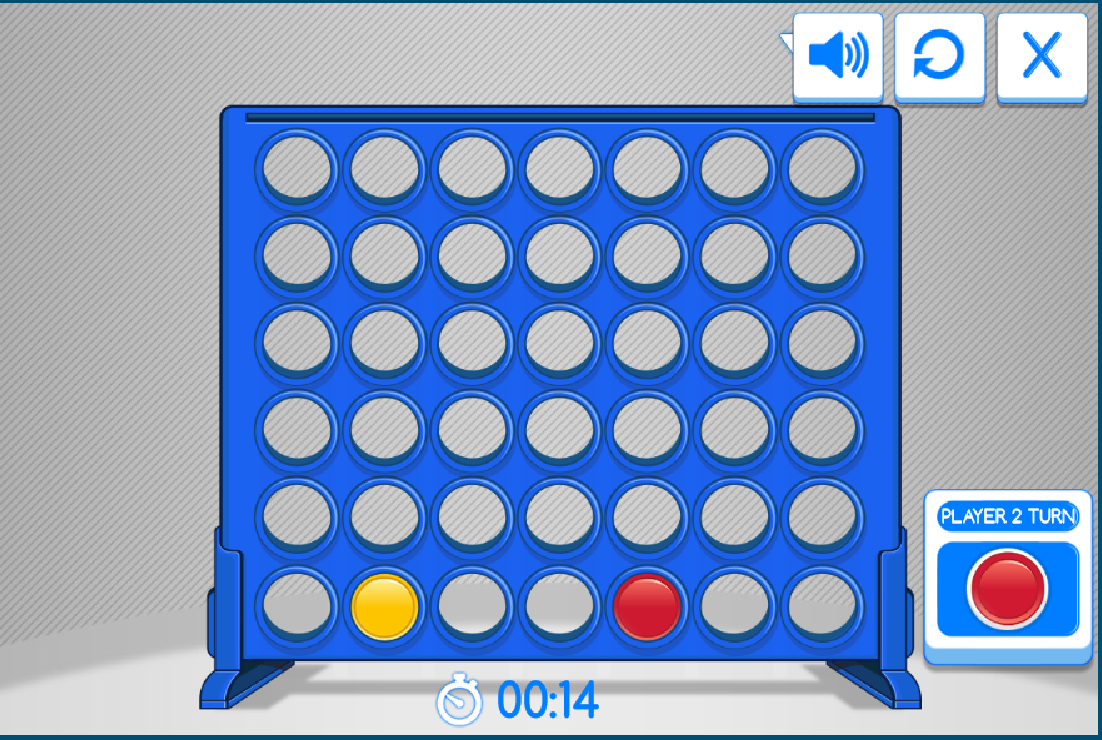
\includegraphics[width=\linewidth]{2}

    
    \section{}
    \subsection{}
    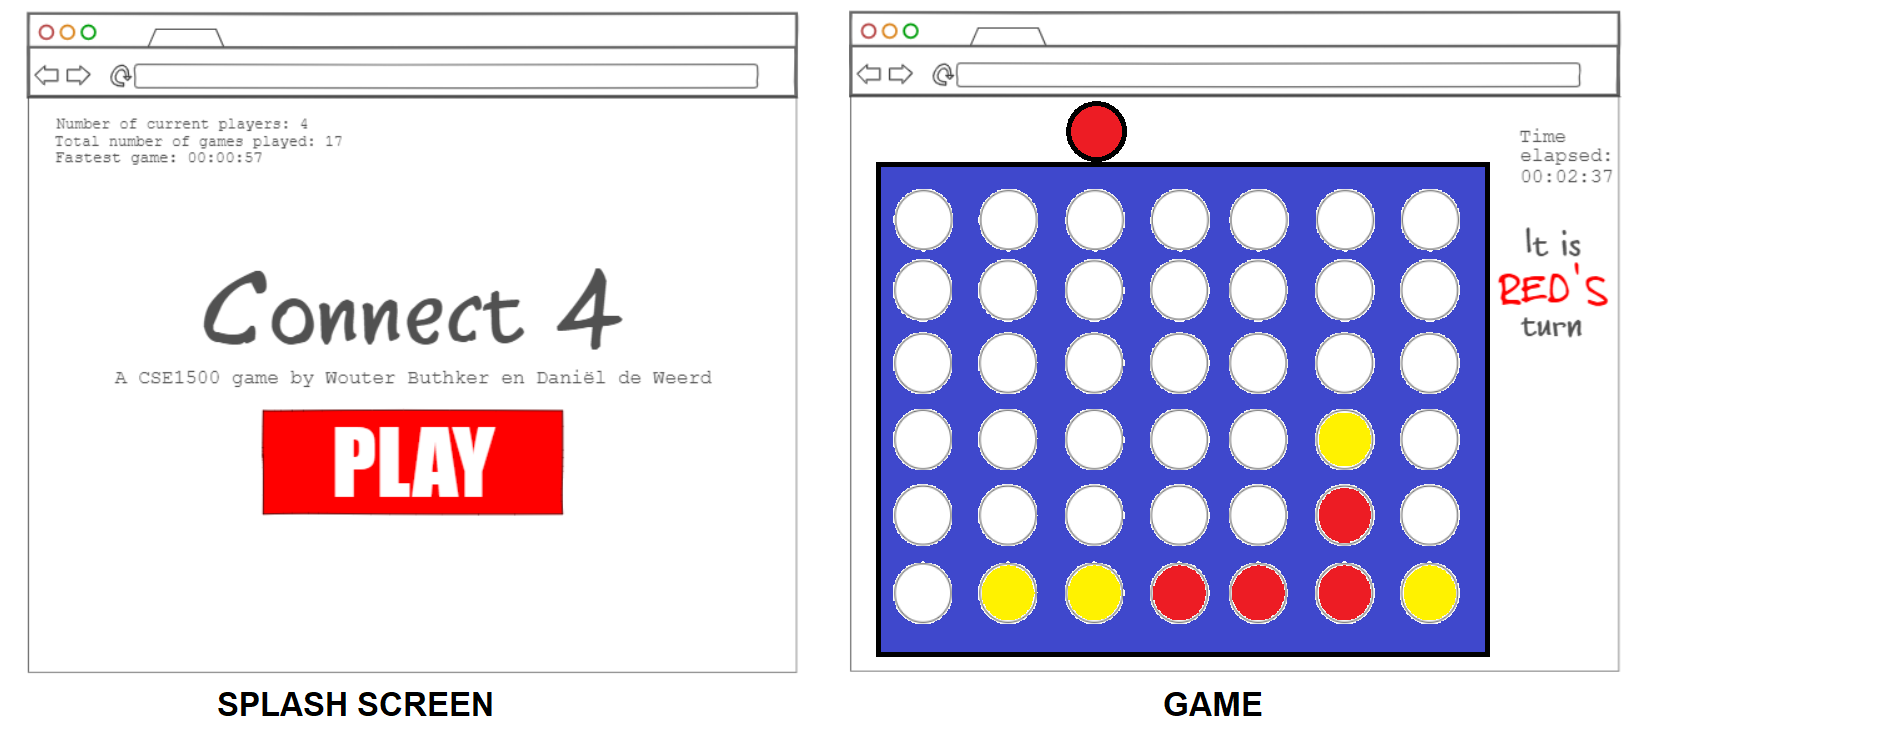
\includegraphics[width=\linewidth]{screens}
    




\end{document}
